% Bagian Hasil Percobaan
\section*{Hasil Percobaan} % Jika ada hasil percobaan

Hasil percobaan yang diperoleh adalah sebagai berikut:

\begin{enumerate}

    \item \textbf{Hasil Konfigurasi Router}
    
    \begin{figure}[H]
        \centering
        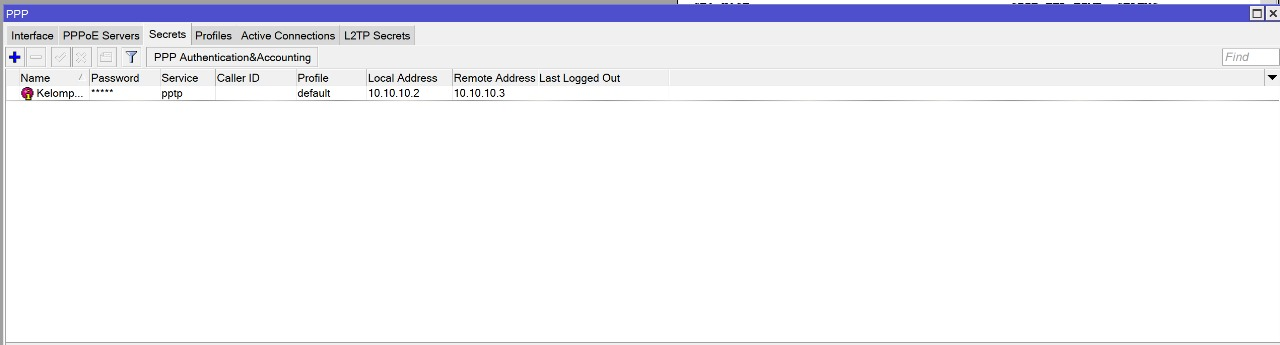
\includegraphics[width=0.9\textwidth]{img/konfigurasi_1.jpeg}
        \caption{Konfigurasi Router}
        \label{fig:konfigurasi_awal}
    \end{figure}

    \begin{figure}[H]
        \centering
        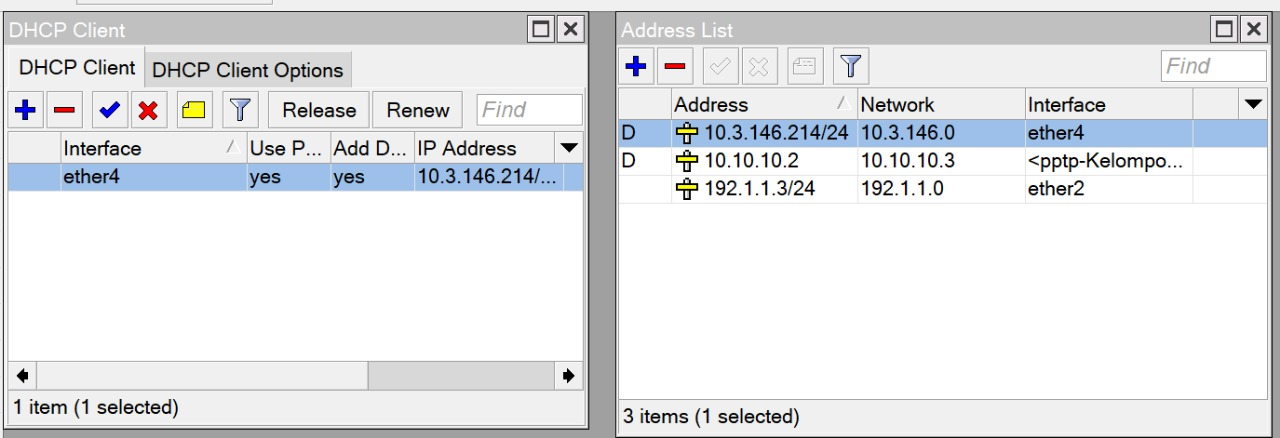
\includegraphics[width=0.9\textwidth]{img/konfigurasi_2.jpeg}
        \caption{Konfigurasi Router}
        \label{fig:konfigurasi_akhir}
    \end{figure}

    \item \textbf{Hasil Pengujian Koneksi PC 1 ke PC 2}
    
    \begin{figure}[H]
        \centering
        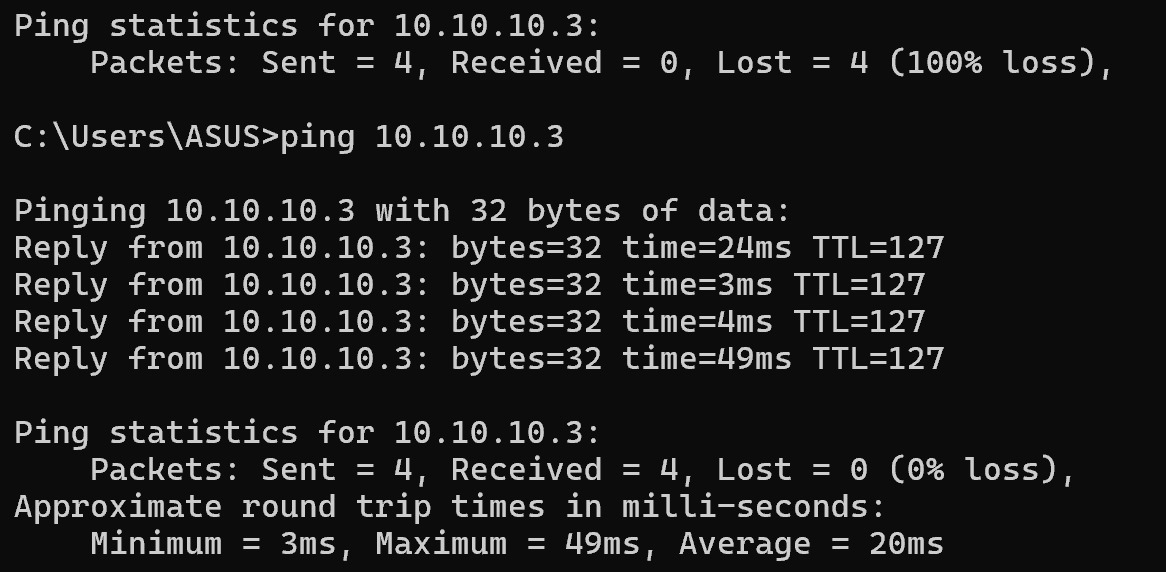
\includegraphics[width=0.7\textwidth]{img/hasil_pc1.jpeg}
        \caption{Ping PC 1 -> PC 2}
        \label{fig:pengujian_koneksi_pc1}
    \end{figure}

    \item \textbf{Hasil Pengujian Koneksi PC 2 ke PC 1}
    
    \begin{figure}[H]
        \centering
        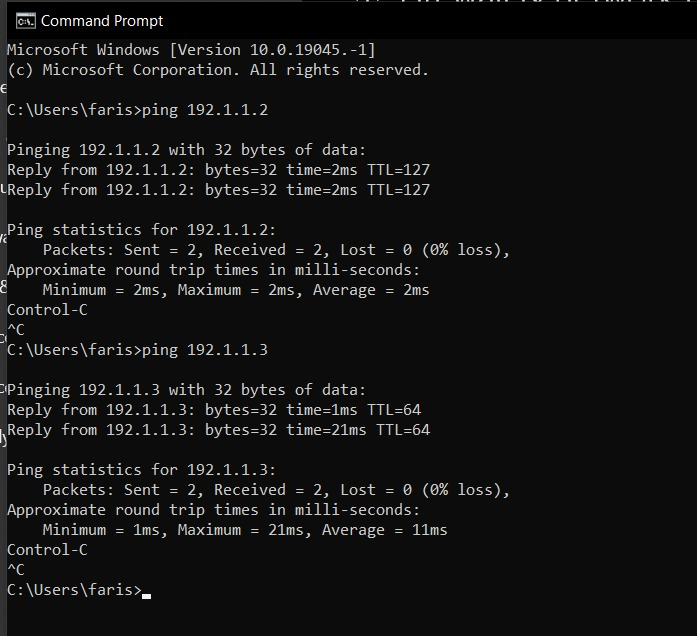
\includegraphics[width=0.7\textwidth]{img/hasil_pc2.jpeg}
        \caption{Ping PC 2 -> PC 1}
        \label{fig:pengujian_koneksi_pc2}
    \end{figure}

\end{enumerate}